\documentclass[final]{nesy2026} % [anon] if review else [final]
\usepackage[T1]{fontenc}
\usepackage{longtable}
\usepackage{booktabs}
\usepackage{siunitx}
\usepackage{xcolor}
\usepackage{tikz}
\usepackage{forest}
\usepackage[1-10]{pagesel}
\usetikzlibrary{calc, shapes.geometric, arrows.meta}

\newcommand{\uu}[1]{\underline{#1}}
\newcommand{\bb}[1]{\textbf{#1}}
\newcommand{\ub}[1]{\uu{\bb{#1}}}

\title[Evaluating Concept Grounding on Craftax]{Abstraction and Knowledge in Reinforcement Learning: Evaluating Concept Grounding on Craftax}

\clearauthor{\Name{Max Adamski} \Email{max.adamski@cs.put.poznan.pl}\\\addr Poznań University of Technology, Poland}

\begin{document}

\maketitle

\begin{abstract}
Symbolic reinforcement learning environments like Craftax provide interpretable observations that are ideal for reasoning.
In such gridworlds, tile vectors can be grounded into high-level concepts via an embedding bottleneck to abstract the state space, while encoding task-specific knowledge into them.
We investigate concept grounding with multi-label classification, using human-provided binary propositions as labels and a weighted binary cross-entropy loss to handle imbalance in the tile distribution.
We integrate concept grounding with Proximal Policy Optimization (PPO) via an additional loss term to allow both the classification loss and the PPO loss to influence embeddings.
We evaluate Craftax agents by comparing total episodic rewards (scores), achievement completion rates, and the total number of parameters. Embedding agents show average scores comparable to the baseline, but higher maximum scores, a 2x reduction in total parameters, and better generalization, completing more achievements in a rare level.
Grounded agents are more robust to initial conditions, showing that prior knowledge can stabilize reinforcement learning.
\end{abstract}

\section{Introduction}
\label{sec:intro}

As neuro-symbolic architectures promise improvements in reinforcement learning \citep{acharya2024}, we evaluate a simple embedding and concept grounding method on the challenging Craftax benchmark \citep{matthews2024} to gain insight into the role of knowledge in learning.
One source of difficulty in Craftax is its wide variety of grid tiles, which are discovered progressively as gameplay ability improves.
We hypothesize that learning from abstracted inputs increases generalization (H1) and that prior knowledge guides learning (H2).
To test our hypotheses, we force agents to generalize across tiles using a compression bottleneck, and we combine the PPO loss \citep{schulman2017} with an auxiliary multi-label classification loss to ground tile embeddings in an expert-defined taxonomy.

More expressive Logic Tensor Networks \citep{serafini2016} have been used to inject prior knowledge and improve shape recognition through symbolic abstraction, although in simpler gridworlds \citep{badreddine2019,amador2025}. 
Concept Bottleneck Models (CBMs) represent an alternative approach to integrating human-defined concepts with neural networks \citep{koh2020}, having been used to guide reinforcement learning in Atari games to avoid the misalignment problem \citep{delfosse2024}.
In general, symbolic interfaces are considered a key enabler of bidirectional human-AI interaction \citep{kambhampati2022}, for instance, allowing humans to advise explainable reinforcement learning agents in an interactive setting \citep{guan2021}.
While expressive and interactive methods are promising, we focus on evaluating the impact of knowledge on reinforcement learning in a complex environment, using a simple method similar to CBMs.

\section{Methods}
\label{sec:methods}

Consider the encoder-decoder architecture shown in \figureref{fig:architecture}.
It is designed for symbolic gridworld observations consisting of a sequence of tiles $e_1, e_2, \ldots, e_N$, where each tile is an interpretable $C$-dimensional vector ($x$), and each dimension is either binary or fuzzy ($0 \le x_i \le 1$).
The encoder is a neural network mapping tile vectors to $E$-dimensional tile embeddings ($z$), and the decoder network maps embeddings to $D$-dimensional logits, which become concept probabilities ($\hat y$) after applying the sigmoid function.
The ground truth ($y$) is computed from original tile features ($x$), using expert-provided binary or fuzzy logic propositions.
The embeddings are optimized to predict concepts, and they introduce a compression bottleneck when $E < C$.
After independently preprocessing each tile, embeddings $e_1', e_2', \ldots, e_N'$ are used as the input of the downstream networks.

\begin{figure}[htbp]
    \centering
    \resizebox{0.8\textwidth}{!}{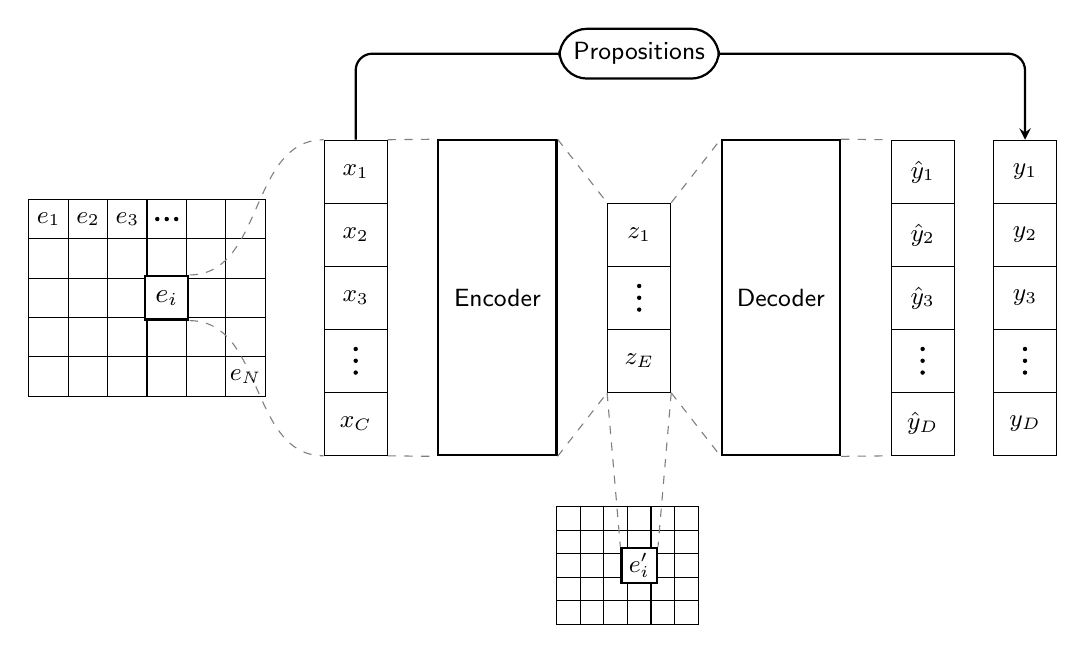
\begin{tikzpicture}[
    font=\sffamily\small,
    cell/.style={rectangle, draw, minimum size=5mm, inner sep=0pt},
    smallcell/.style={rectangle, draw, minimum size=3mm, inner sep=0pt},
    block/.style={rectangle, draw=black, fill=white, thick, minimum width=1.5cm, inner sep=0pt},
    column/.style={rectangle, draw, minimum size=8mm, inner sep=0pt},
    v_dots/.style={
        column,
        path picture={
            \foreach \i in {-0.15, 0, 0.15}
                \fill (path picture bounding box.center) +(0,\i) circle (0.8pt);
        }
    },
    h_dots/.style={
        cell,
        path picture={
            \foreach \i in {-0.12, 0, 0.12}
                \fill (path picture bounding box.center) +(\i,0) circle (0.8pt);
        }
    }
]

    % --- 1. Input Element Grid ---
    \begin{scope}[shift={(0,0)}]
        \foreach \x in {0,...,5}
            \foreach \y in {0,...,4}
                \node[cell] (e\x\y) at (\x*0.5, -\y*0.5) {};
        
        \node at (e00) {$e_1$};
        \node at (e10) {$e_2$};
        \node at (e20) {$e_3$};
        \node[h_dots] at (e30) {};
        \node[cell, fill=white, scale=1.1, thick] (ei_box) at (e32) {$e_i$};
        \node at (e54) {$e_N$};
    \end{scope}

    % --- 2. Vector X ---
    \begin{scope}[shift={(3.9, -1.0)}] 
        \node[column] (x1) at (0, 1.6) {$x_1$};
        \node[column] (x2) at (0, 0.8) {$x_2$};
        \node[column] (x3) at (0, 0) {$x_3$};
        \node[v_dots] (xdots) at (0, -0.8) {};
        \node[column] (xc) at (0, -1.6) {$x_C$};
    \end{scope}

    % --- 3. Encoder Block ---
    \node[block, minimum height=4cm] (encoder) at (5.7, -1.0) {Encoder};

    % --- 4. Latent Representation H ---
    \begin{scope}[shift={(7.5, -1.0)}]
        \node[column] (h1) at (0, 0.8) {$z_1$};
        \node[v_dots] (hdots) at (0, 0) {};
        \node[column] (he) at (0, -0.8) {$z_E$};
    \end{scope}

    % --- 5. Smaller Output Grid ---
    \begin{scope}[shift={(6.6, -3.8)}]
        \foreach \x in {0,...,5}
            \foreach \y in {0,...,4}
                \node[smallcell] (em\x\y) at (\x*0.3, -\y*0.3) {};
        
        \node[rectangle, draw=black, fill=white, thick, minimum size=4.5mm, inner sep=0pt] (eip) at (em32) {$e_i'$};
    \end{scope}

    % --- 7. Decoder Block ---
    \node[block, minimum height=4cm] (decoder) at (9.3, -1.0) {Decoder};

    % --- 8. Output Vectors ---
    \begin{scope}[shift={(11.1, -1.0)}]
        \node[column] (yh1) at (0, 1.6) {$\hat{y}_1$};
        \node[column] (yh2) at (0, 0.8) {$\hat{y}_2$};
        \node[column] (yh3) at (0, 0) {$\hat{y}_3$};
        \node[v_dots] (yhdots) at (0, -0.8) {};
        \node[column] (yhd) at (0, -1.6) {$\hat{y}_D$};
    \end{scope}

    \begin{scope}[shift={(12.4, -1.0)}]
        \node[column] (y1) at (0, 1.6) {$y_1$};
        \node[column] (y2) at (0, 0.8) {$y_2$};
        \node[column] (y3) at (0, 0) {$y_3$};
        \node[v_dots] (ydots) at (0, -0.8) {};
        \node[column] (yd) at (0, -1.6) {$y_D$};
    \end{scope}

    % --- 9. Connections ---
    \draw[dashed, gray] (ei_box.north east) to [out=0, in=180] (x1.north west);
    \draw[dashed, gray] (ei_box.south east) to [out=0, in=180] (xc.south west);
    \draw[dashed, gray] (x1.north east) -- (encoder.north west);
    \draw[dashed, gray] (xc.south east) -- (encoder.south west);
    \draw[dashed, gray] (encoder.north east) -- (h1.north west);
    \draw[dashed, gray] (encoder.south east) -- (he.south west);
    \draw[dashed, gray] (h1.north east) -- (decoder.north west);
    \draw[dashed, gray] (he.south east) -- (decoder.south west);
    \draw[dashed, gray] (decoder.north east) -- (yh1.north west);
    \draw[dashed, gray] (decoder.south east) -- (yhd.south west);
    \draw[dashed, gray] (he.south west) -- (eip.north west);
    \draw[dashed, gray] (he.south east) -- (eip.north east);

    % --- 10. Overhead "Through" Path ---
    \draw[thick, ->, >=stealth, rounded corners=6pt] 
        (x1.north) -- (3.9, 2.1) -- (12.4, 2.1) -- (y1.north);

    \node[draw=black, rounded corners=10pt, inner sep=5pt, thick, fill=white] at (7.5, 2.1) {Propositions};

\end{tikzpicture}}
    \caption{Concept grounding architecture for gridworlds}
    \label{fig:architecture}
\end{figure}

In \equationref{eq:concept_loss}, we define the loss that the encoder and decoder must minimize so that embeddings predict concepts.
It is a standard binary cross-entropy loss for imbalanced multi-label classification, averaged across labels. The concept loss is scaled by the hyperparameter $\lambda_{\mathcal K}$ and is added to the PPO loss ($\mathcal L = \mathcal{L_{PPO}} + \lambda_{\mathcal K} \mathcal{L_K}$).

\begin{equation}
  \mathcal{L_K} = \frac{1}{D} \sum_{i=1}^D \left[ -w_i y_i \log(\hat{y}_i) - (1 - y_i) \log(1 - \hat{y}_i) \right] \label{eq:concept_loss}
\end{equation}

In \equationref{eq:concept_weight}, we define the weighting scheme. Assuming imbalance in concept value distributions, each example is weighted inversely to the mean concept value in the minibatch ($\bar y_i$).
For binary concepts, the weight is proportional to the number of negative examples in the minibatch ($n_i^-$), and inversely proportional to the number of positive examples ($n_i^+$).
Negative examples are not weighted, so division by zero is avoided.

\begin{equation}
  w_i = \frac{1}{\bar y_i} - 1 = \frac{n_i^-}{n_i^+} \label{eq:concept_weight}
\end{equation}

In \figureref{fig:taxonomy}, we propose a taxonomy of Craftax tiles that contains our knowledge of the game.
Craftax observations mainly consist of 83-dimensional tiles $e_1, e_2, \ldots, e_{99}$, which are interpreted as an $11 \times 9$ grid.
For convenience, we assign lowercase names to dimensions $x_1, \ldots, x_{83}$, and capitalized names to concepts $y_1, \ldots, y_{19}$.
Among others, we define the \emph{Ranged} concept, grouping tiles occupied by similar enemies, with the binary proposition $\emph{Ranged} \iff \emph{skeleton} \lor \emph{orc~mage} \lor \emph{gnome~archer}$. We also define concepts in terms of other concepts, like $\emph{Enemies} \iff \emph{Ranged} \lor \emph{Melee}$, and using inequalities, like $\emph{Dark} \iff \emph{light~level} < 0.05$. We implement these propositions as efficient tensor operations.

\begin{figure}[htbp]
  \floatconts{fig:taxonomy}
  {\caption{Proposed taxonomy for Craftax}}
  {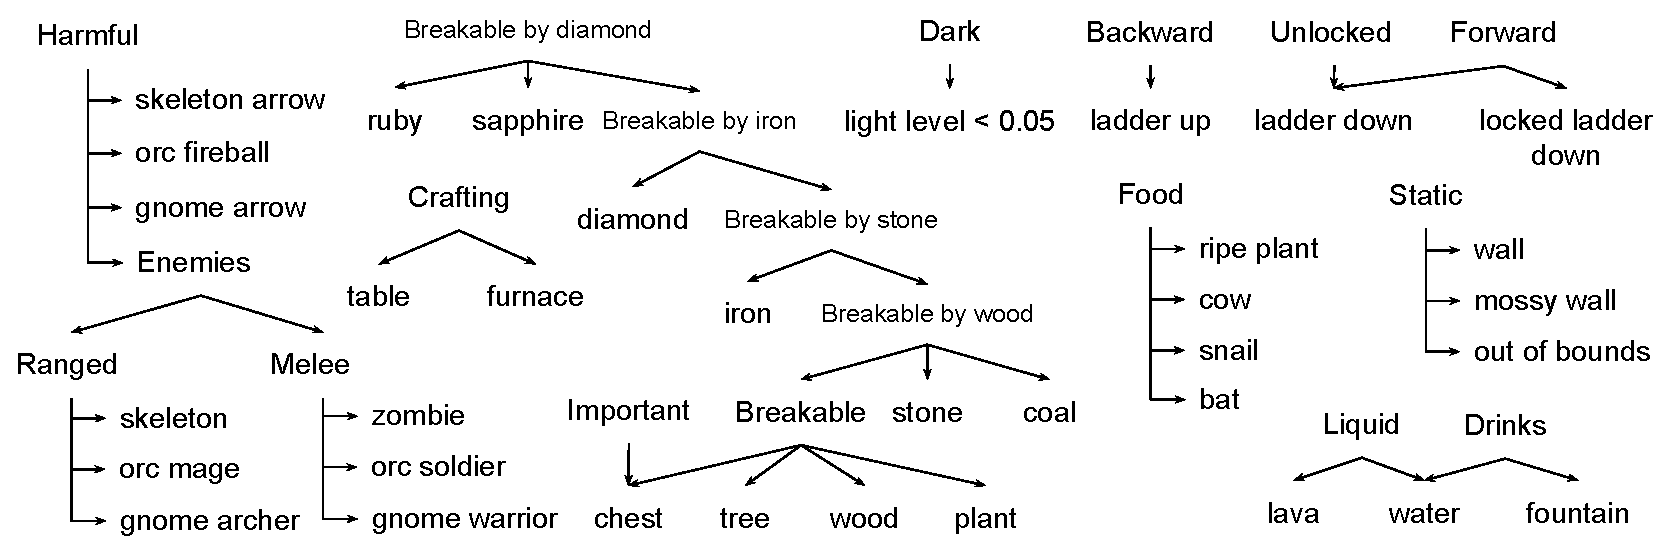
\includegraphics[width=\linewidth]{include/taxonomy.pdf}}
\end{figure}


We compare the concept grounding architecture against a baseline non-recursive PPO method.
To test H1, we separate the effect of abstraction introduced by the compression bottleneck, and to test H2 we remove guidance with prior knowledge by replacing supervised concept classification with self-supervised tile reconstruction.
In total, we evaluate the following four methods:

\begin{enumerate}
\item \textbf{Baseline}: the agent learns from raw observations.
\item \textbf{Compression}: the encoder compresses tiles, but the decoder is removed.
\item \textbf{Autoencoder}: compression, but a symmetric decoder reconstructs tiles ($y_i = x_i$).
\item \textbf{Grounding}: compression, but a single layer decoder grounds tiles in our taxonomy.
\end{enumerate}

For each method, we train 20 agents for 500 million steps, starting from different random seeds.
Notably, we use the same concept loss scale ($\lambda_{\mathcal K} = 0.5$) for both the autoencoder and grounding methods.
We then evaluate each agent for 100 thousand episodes across 4096 different worlds.
During evaluation, agents simply sample actions from their learned policy, which does not require the decoder.
After an episode ends, we record the score, defined as the normalized total episodic reward, and the binary vector of completed achievements.
For each agent, we divide the number of evaluation episodes where a given achievement is completed, by the total number of evaluation episodes, to get the achievement rate.

\section{Results}
\label{sec:results}

\tableref{tab:methods} shows the tile dimension, the total agent parameter count (in millions), and the average and maximum score of each method (mean and standard deviation across agents).
Embeddings do not change the average score, but they do increase the maximum score.
The twofold reduction in agent parameter count is explained in \appendixref{apd:model_details}.

\begin{table}[htbp]
\floatconts{tab:methods}
{\caption{Evaluation summary}}
{\begin{tabular}{lcccc}
\toprule
\textbf{Method} & \textbf{Tile Dim.} & \textbf{Params} & \textbf{Avg. Score} & \textbf{Max. Score} \\
\midrule
Baseline    & 83 & 9.54M & $11.62\% \pm 0.13\%$ & $22.75\% \pm 0.41\%$ \\
Compression & 32 & 4.39M & $11.82\% \pm 0.19\%$ & $25.24\% \pm 1.00\%$ \\
Autoencoder & 32 & 4.42M & $11.77\% \pm 0.17\%$ & $25.27\% \pm 1.20\%$ \\
Grounding   & 32 & 4.39M & $11.87\% \pm 0.18\%$ & $26.42\% \pm 1.15\%$ \\
\bottomrule
\end{tabular}}
\end{table}


In \figureref{fig:analogous_achievements}, we show the completion rates for analogous achievements in common and rare scenarios (mean across agents and individual values).
Embeddings slightly increase achievement rates after entering a common level, and greatly increase analogous achievement rates after entering a rare level.\footnote{To compare rates across levels, we show rescaled achievement rates $P(A|B) = P(A)/P(B)$, where completing achievement $A$ requires first completing achievement $B$.}
All grounded agents learn to complete analogous achievements at similar rates in both levels, while a few compression and many autoencoder agents show degraded performance in the rare level.

\begin{figure}[htbp]
  \floatconts{fig:analogous_achievements}
  {\caption{Completion rates for analogous achievements}}
  {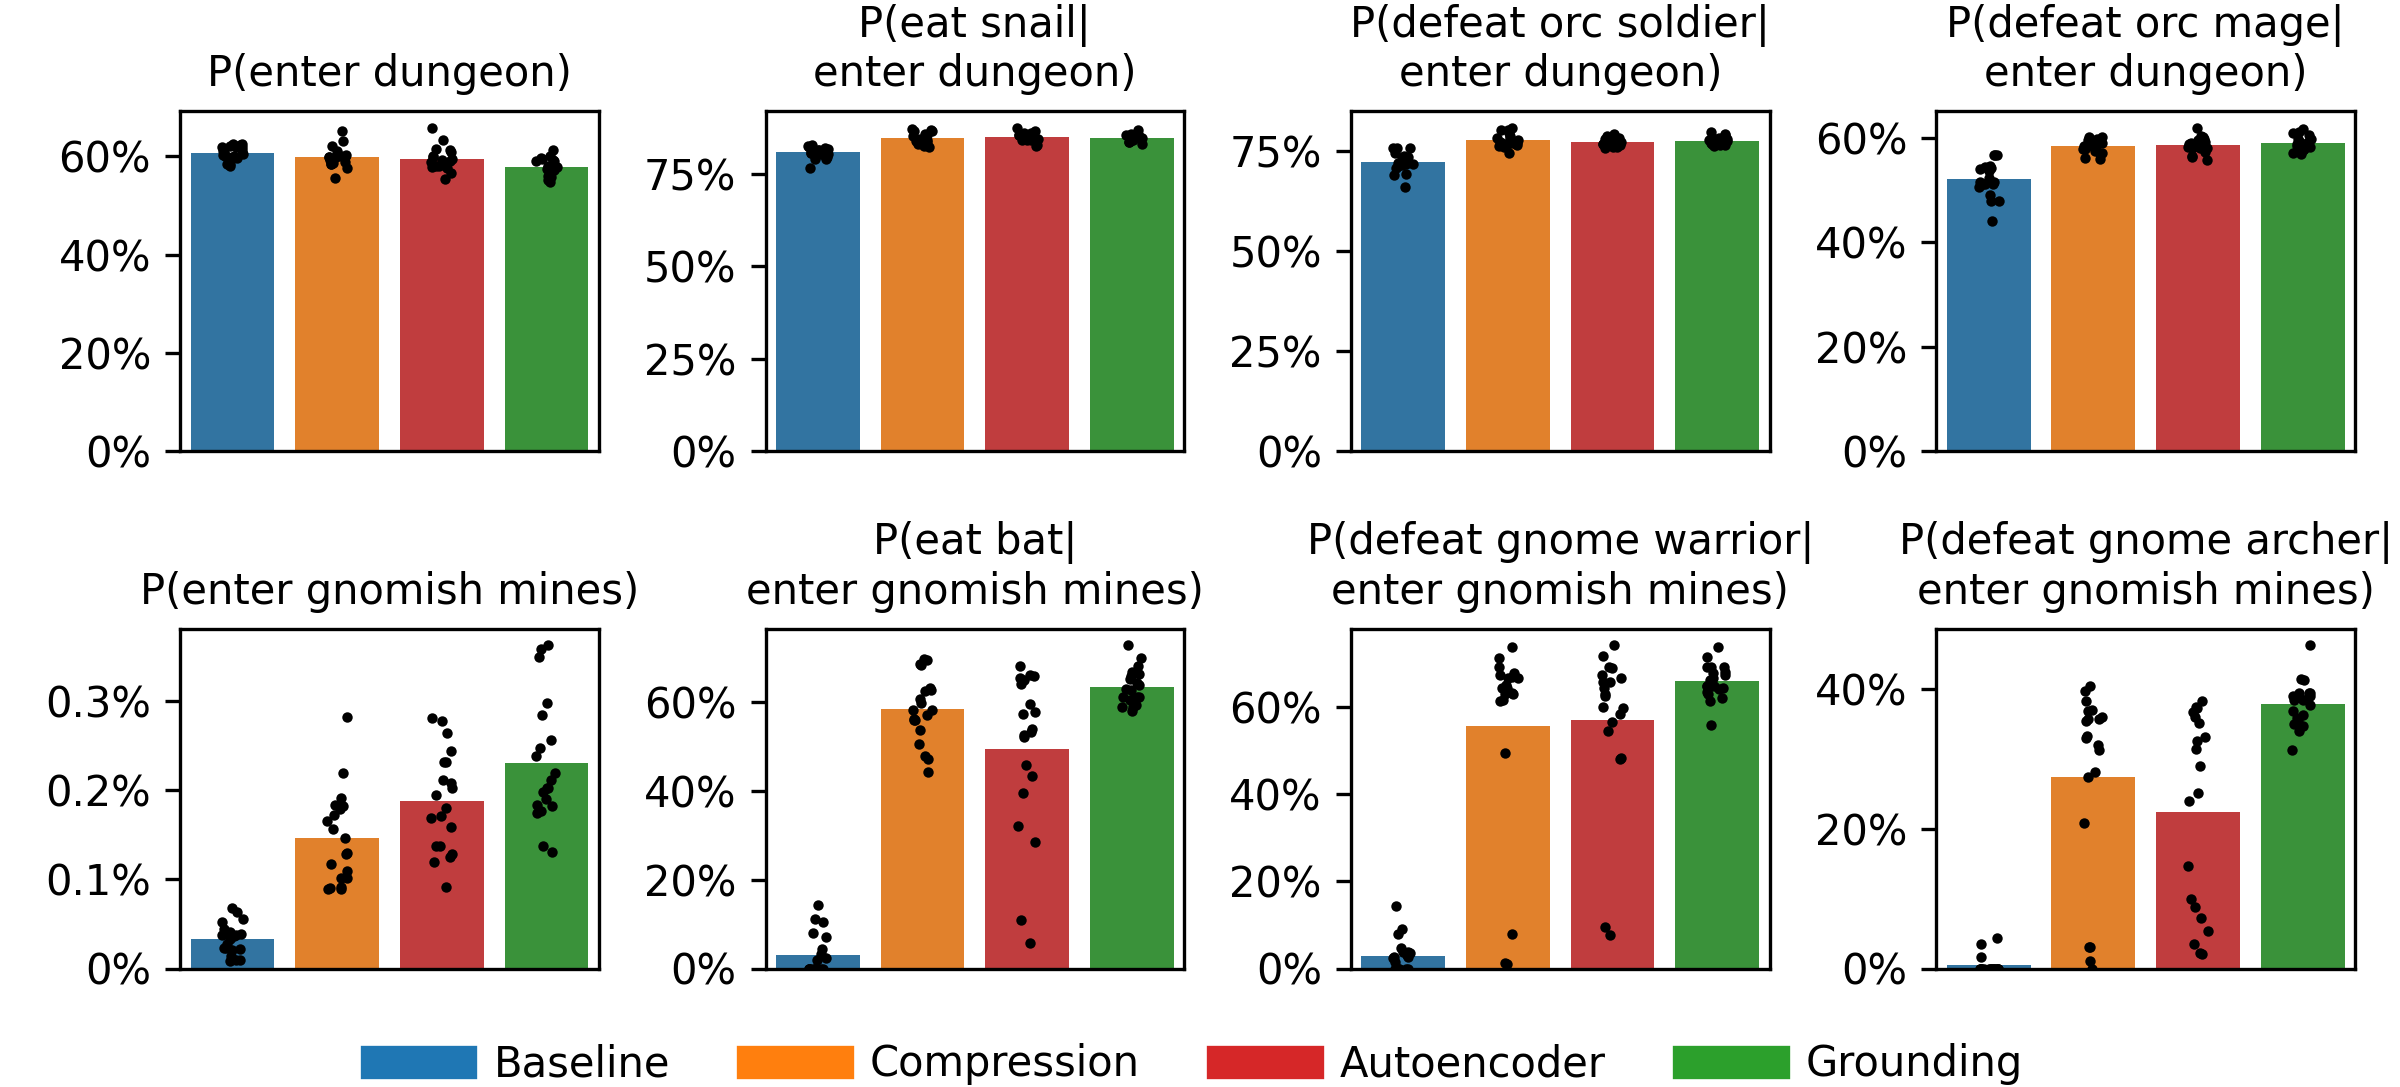
\includegraphics[width=\linewidth]{include/abtest_analogous.png}}
\end{figure}


In \figureref{fig:iron_achievements}, we show that compression degrades performance for most agents on two common achievements and one rare achievement, but grounding limits the effect.

\begin{figure}[htbp]
  \floatconts{fig:iron_achievements}
  {\caption{Completion rates for iron-related achievements}}
  {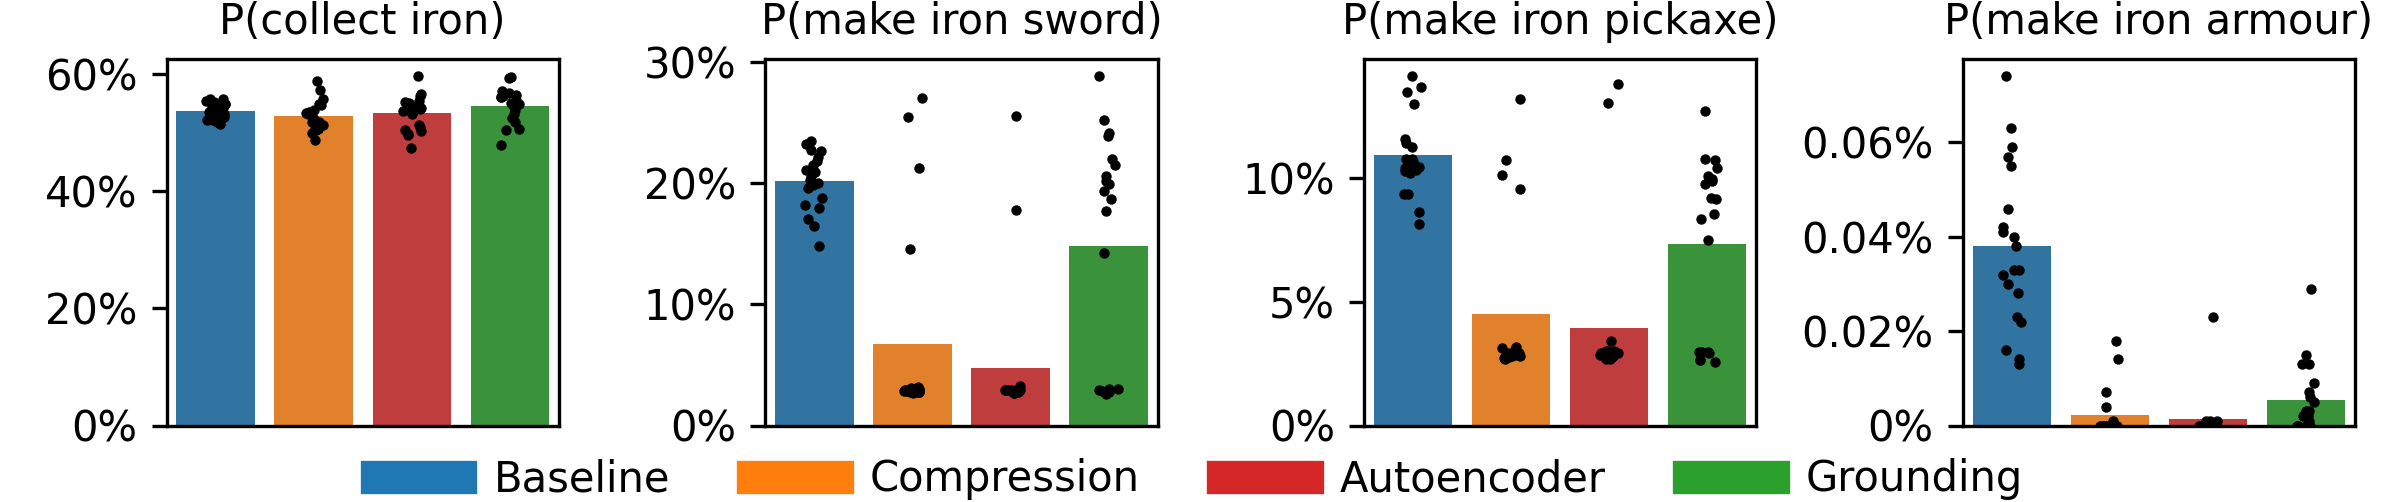
\includegraphics[width=\linewidth]{include/abtest_iron.png}}
\end{figure}

\section{Conclusions}
\label{sec:conclusions}

The average score on Craftax remains at the level of the baseline for all of the investigated embedding methods.
However, compressing tiles in Craftax greatly decreased parameter counts and allowed agents to generalize across tiles to complete analogous achievements regardless of level and tile rarity.
Additionally, concept grounding stabilized learning with prior knowledge of the symbolic environment.

The difference between compression and concept grounding shows that jointly learning multi-label classification for an expert-designed taxonomy can have a stabilizing effect and can even partially recover performance lost in bottlenecks.
Conversely, the autoencoder method shows that learning to reconstruct tiles does not stabilize learning in a symbolic environment where tiles do not contain visual patterns.

We see that learning from abstracted inputs can increase generalization (H1), as supported by significant improvements in completion rates for a class of Craftax achievements and dramatic improvements in a rare level where new tiles are introduced.
We also find that prior knowledge can guide learning (H2), as shown in a rare level where unguided agents can fail to complete analogous achievements simply because of a random seed, as well as in a common level where most unguided embedding agents fail to complete iron-related achievements, while many grounding agents succeed.

Reinforcement learning with PPO can be unstable, as shown by the high variance of average scores across training runs on some Atari games \citep{schulman2017}, and as we see with embedding agents on some Craftax achievements.
In this context, we consider concept grounding to be a semantic regularizer, as it reduces sensitivity to random seeds.
However, it has limited applicability by assuming a symbolic environment and requiring additional modeling and knowledge engineering.

Future work may investigate more expressive architectures and knowledge bases with recurrent Craftax models; though they achieve higher scores, they remain insufficient to fully solve this benchmark, even on a large 10 billion step budget.

\acks{We thank Jędrzej Potoniec and Wojciech Kotłowski for their support, and the Poznań University of Technology for GPU access.}

\bibliography{paper}

\appendix

\section{Architectural details}\label{apd:model_details}

Our downstream actor and critic networks have 3 layers, each with 512 neurons and ReLU activation.
Craftax has an 8268-dimensional observation space ($9 \times 11 \times 83$ for tiles and 51 for global state), so the actor and critic contain $8268 \times 512 \times 2$ weights in their first layers, which accounts for the majority of agent parameters.
The encoder accepts 83-dimensional inputs, consists of 3 layers, each with 83 neurons and ReLU activation, and outputs 32-dimensional embeddings.
Embedding the tiles results in a 3219-dimensional observation space, which proportionately reduces the number of weights in the first layers of the actor and critic.

\section{Training details}\label{apd:training_details}

We train each agent for 500 million steps across 1024 different environments.
We perform rollouts for 64 steps, resulting in batches of 65536 steps.\footnote{We prevent illegal actions during rollouts by setting their logits to $-\infty$ before applying softmax.}
Each batch is divided into 16 minibatches of 4096 steps.
Notably, each step contains an observation with 99 tiles, meaning that the encoder is trained on large minibatches of tiles.
To prevent exploding gradients, we apply gradient clipping with a maximum norm of 1.

In \figureref{fig:train_plots}, we show achievement rates during training (mean and standard deviation across agents). To reduce noise, we apply a running average with a window size of 40 batches, resulting in 190 data points per plot.

We optimize the agent end-to-end with AdamW, with a constant learning rate throughout training ($\eta = 2\cdot10^{-4}$), and using default values for the remaining optimizer hyperparameters.\footnote{See \url{https://docs.pytorch.org/docs/2.9/generated/torch.optim.AdamW.html}}
We reuse each batch for 3 epochs to improve sample efficiency, and we use the same values as \cite{matthews2024} for generalized advantage estimation ($\lambda = 0.8$), the discount factor ($\gamma = 0.99$), and PPO hyperparameters for policy update clipping ($\epsilon = 0.2$), scaling the value loss ($c_1 = 0.5$), and scaling the entropy bonus ($c_2 = 0.01$).

\section{Evaluation details}\label{apd:statistical_testing}

We consider a set of 42 achievements.
Because no agents advanced beyond the \emph{gnomish mines} level, we exclude achievements that can only be completed in later levels.
For completeness, we present the evaluation results for all considered achievements in \figureref{fig:eval_plots}.

For each method, we train a population of agents ($n = 20$) using different random seeds.
We then apply the non-parametric, two-sided Mann-Whitney U test to support our claims of statistically significant changes in achievement completion rates relative to the baseline method.
A significant result for a given achievement indicates that the two methods have distinct completion rate distributions, accounting for the effects of random initialization during training and randomness of the environment.

We perform three families of tests, independently comparing the baseline method's achievement rates with those of the compression, autoencoder, and grounding methods.
For each family, we apply the Bonferroni-Holm correction to control the family-wise error rate and reduce the probability of false-positive findings when performing multiple comparisons.

In \tableref{tab:tests}, we report the mean and standard deviation of the achievement rates (in \%) across the baseline agents.
For the embedding methods, we report the change in the mean achievement rate in percentage points ($\Delta$p.p.).
For each achievement, we underline statistically significant changes ($p < 0.05$) and highlight the change that results in the highest mean completion rate, indicating the best embedding method for that metric.
For certain achievements, a negative change is highlighted, which indicates that the baseline outperforms the embedding methods.
To reduce noise, we omit highlighting for achievements with no statistically significant changes.

\begin{figure}[htbp]
  \floatconts{fig:train_plots}
  {\caption{Completion rates for all considered achievements during training}}
  {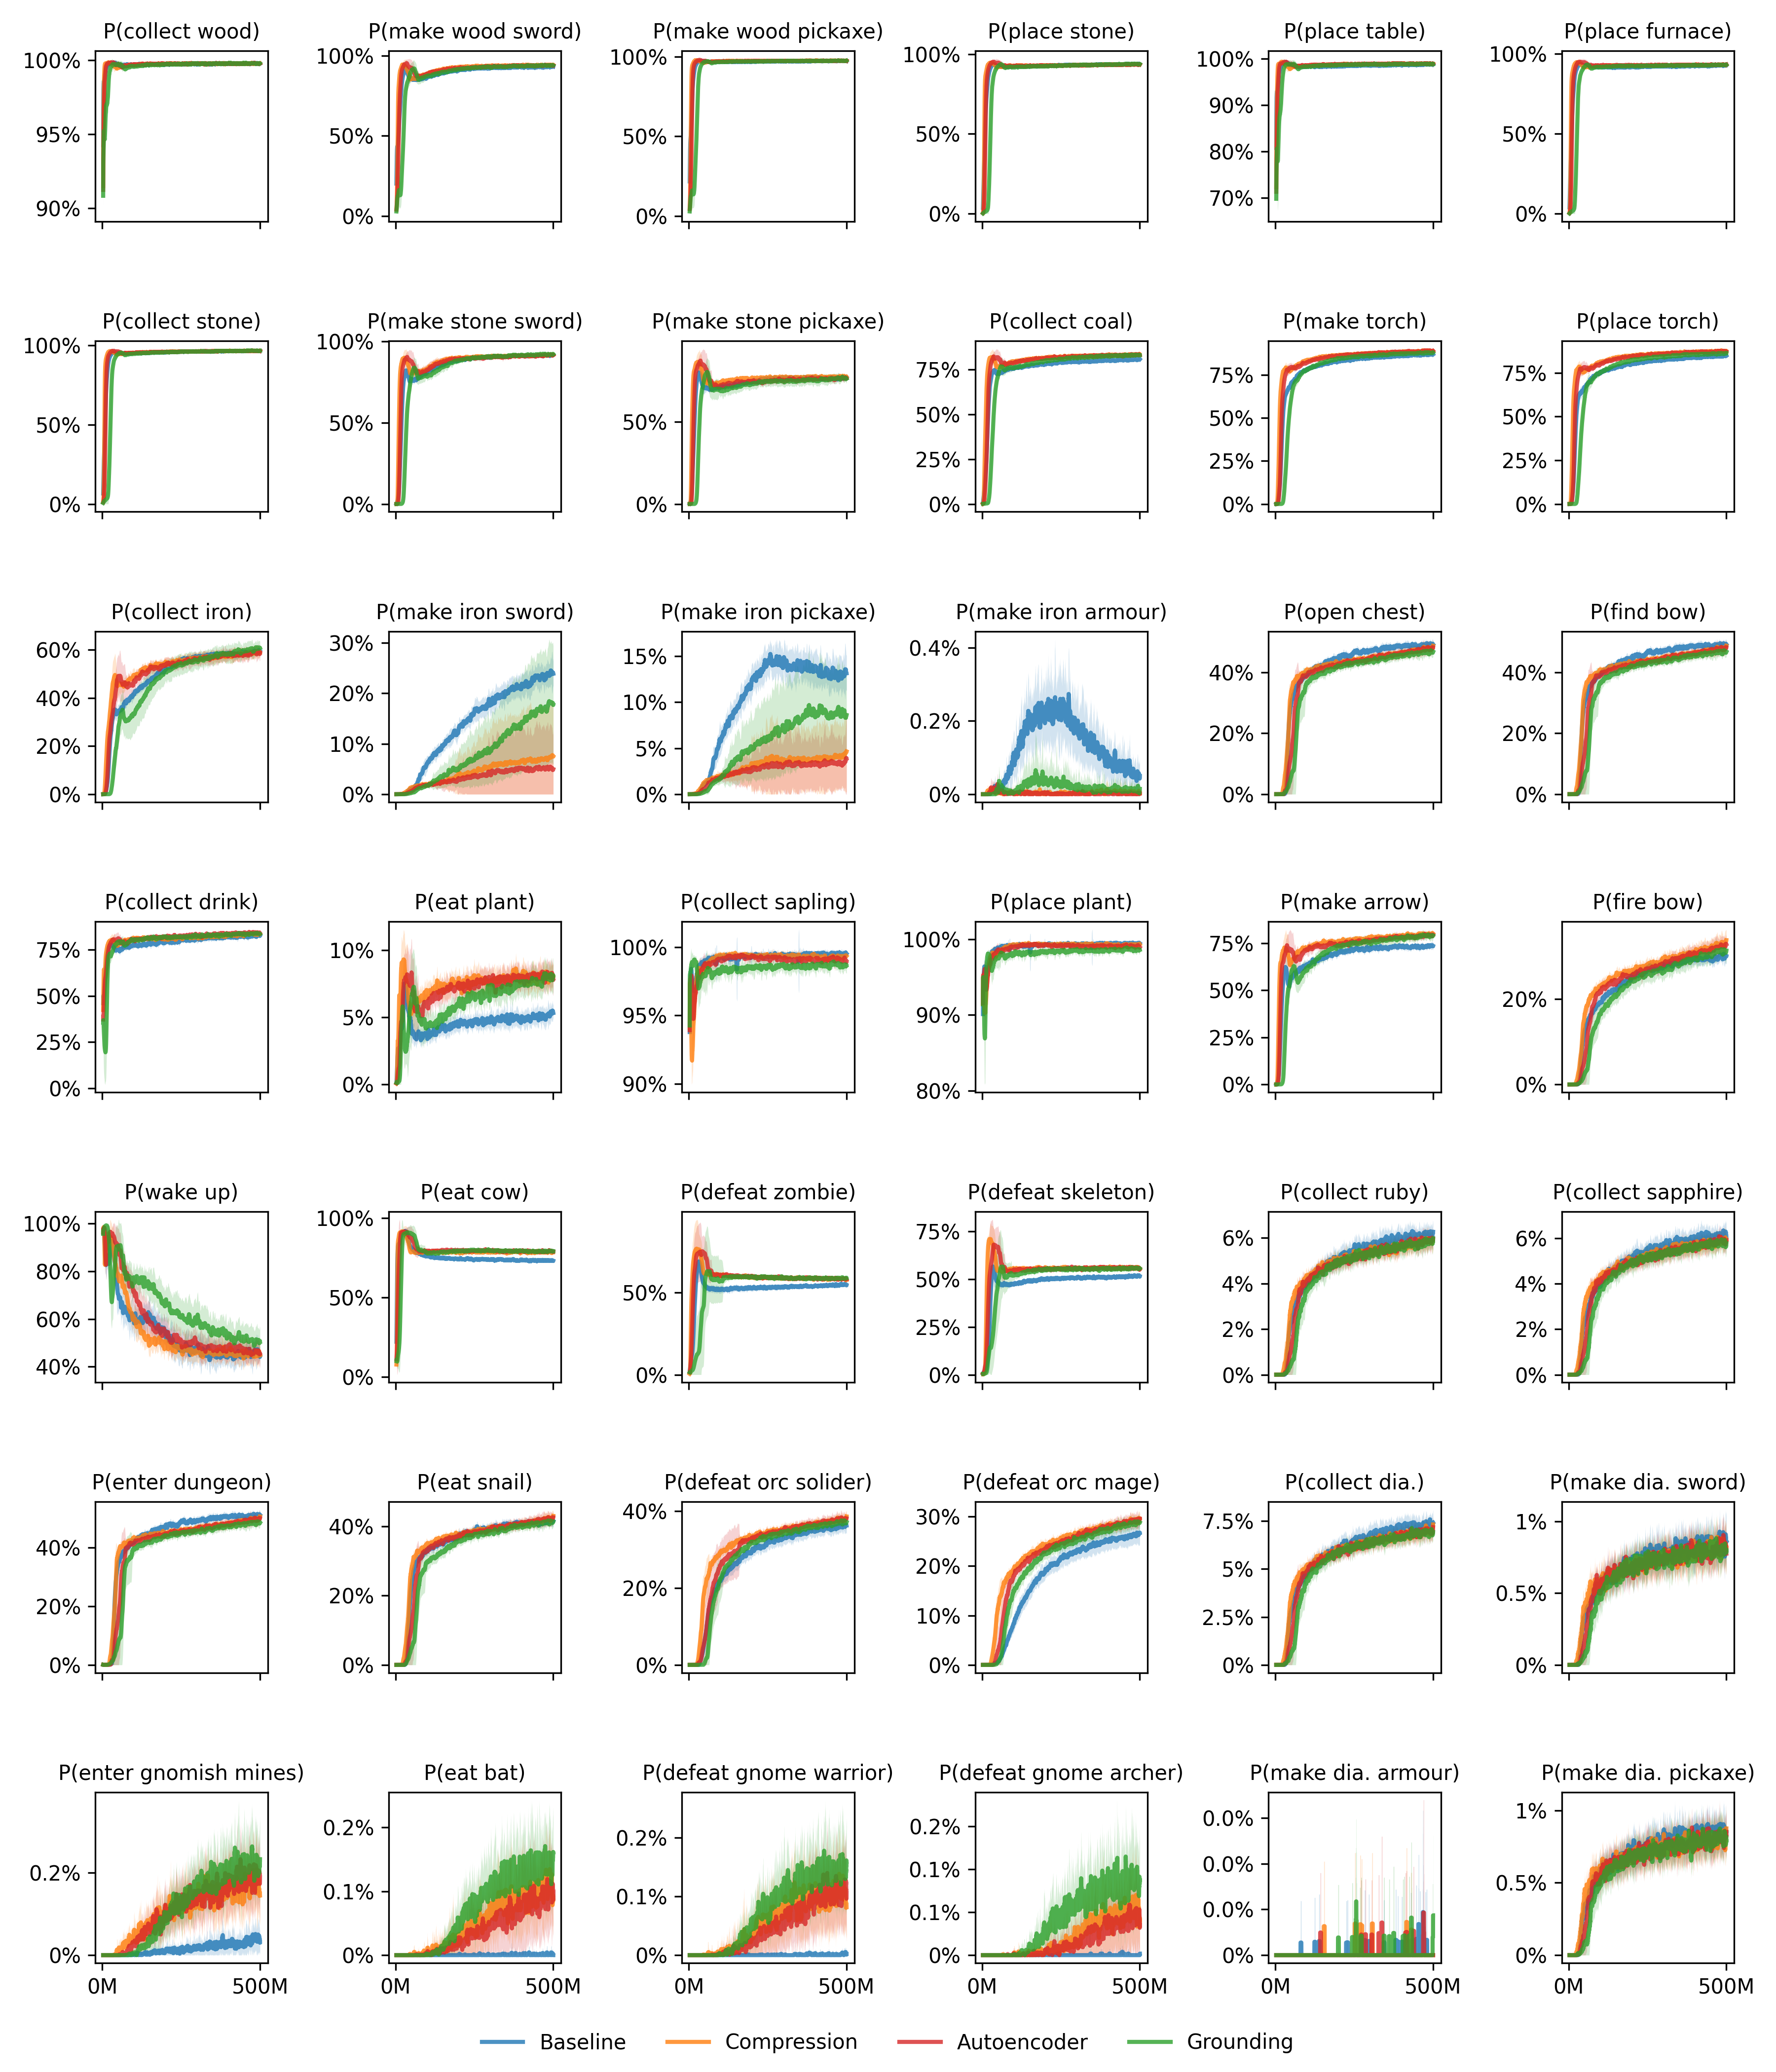
\includegraphics[width=\linewidth]{include/training.png}}
\end{figure}

\begin{figure}[htbp]
  \floatconts{fig:eval_plots}
  {\caption{Evaluation results for all considered achievements}}
  {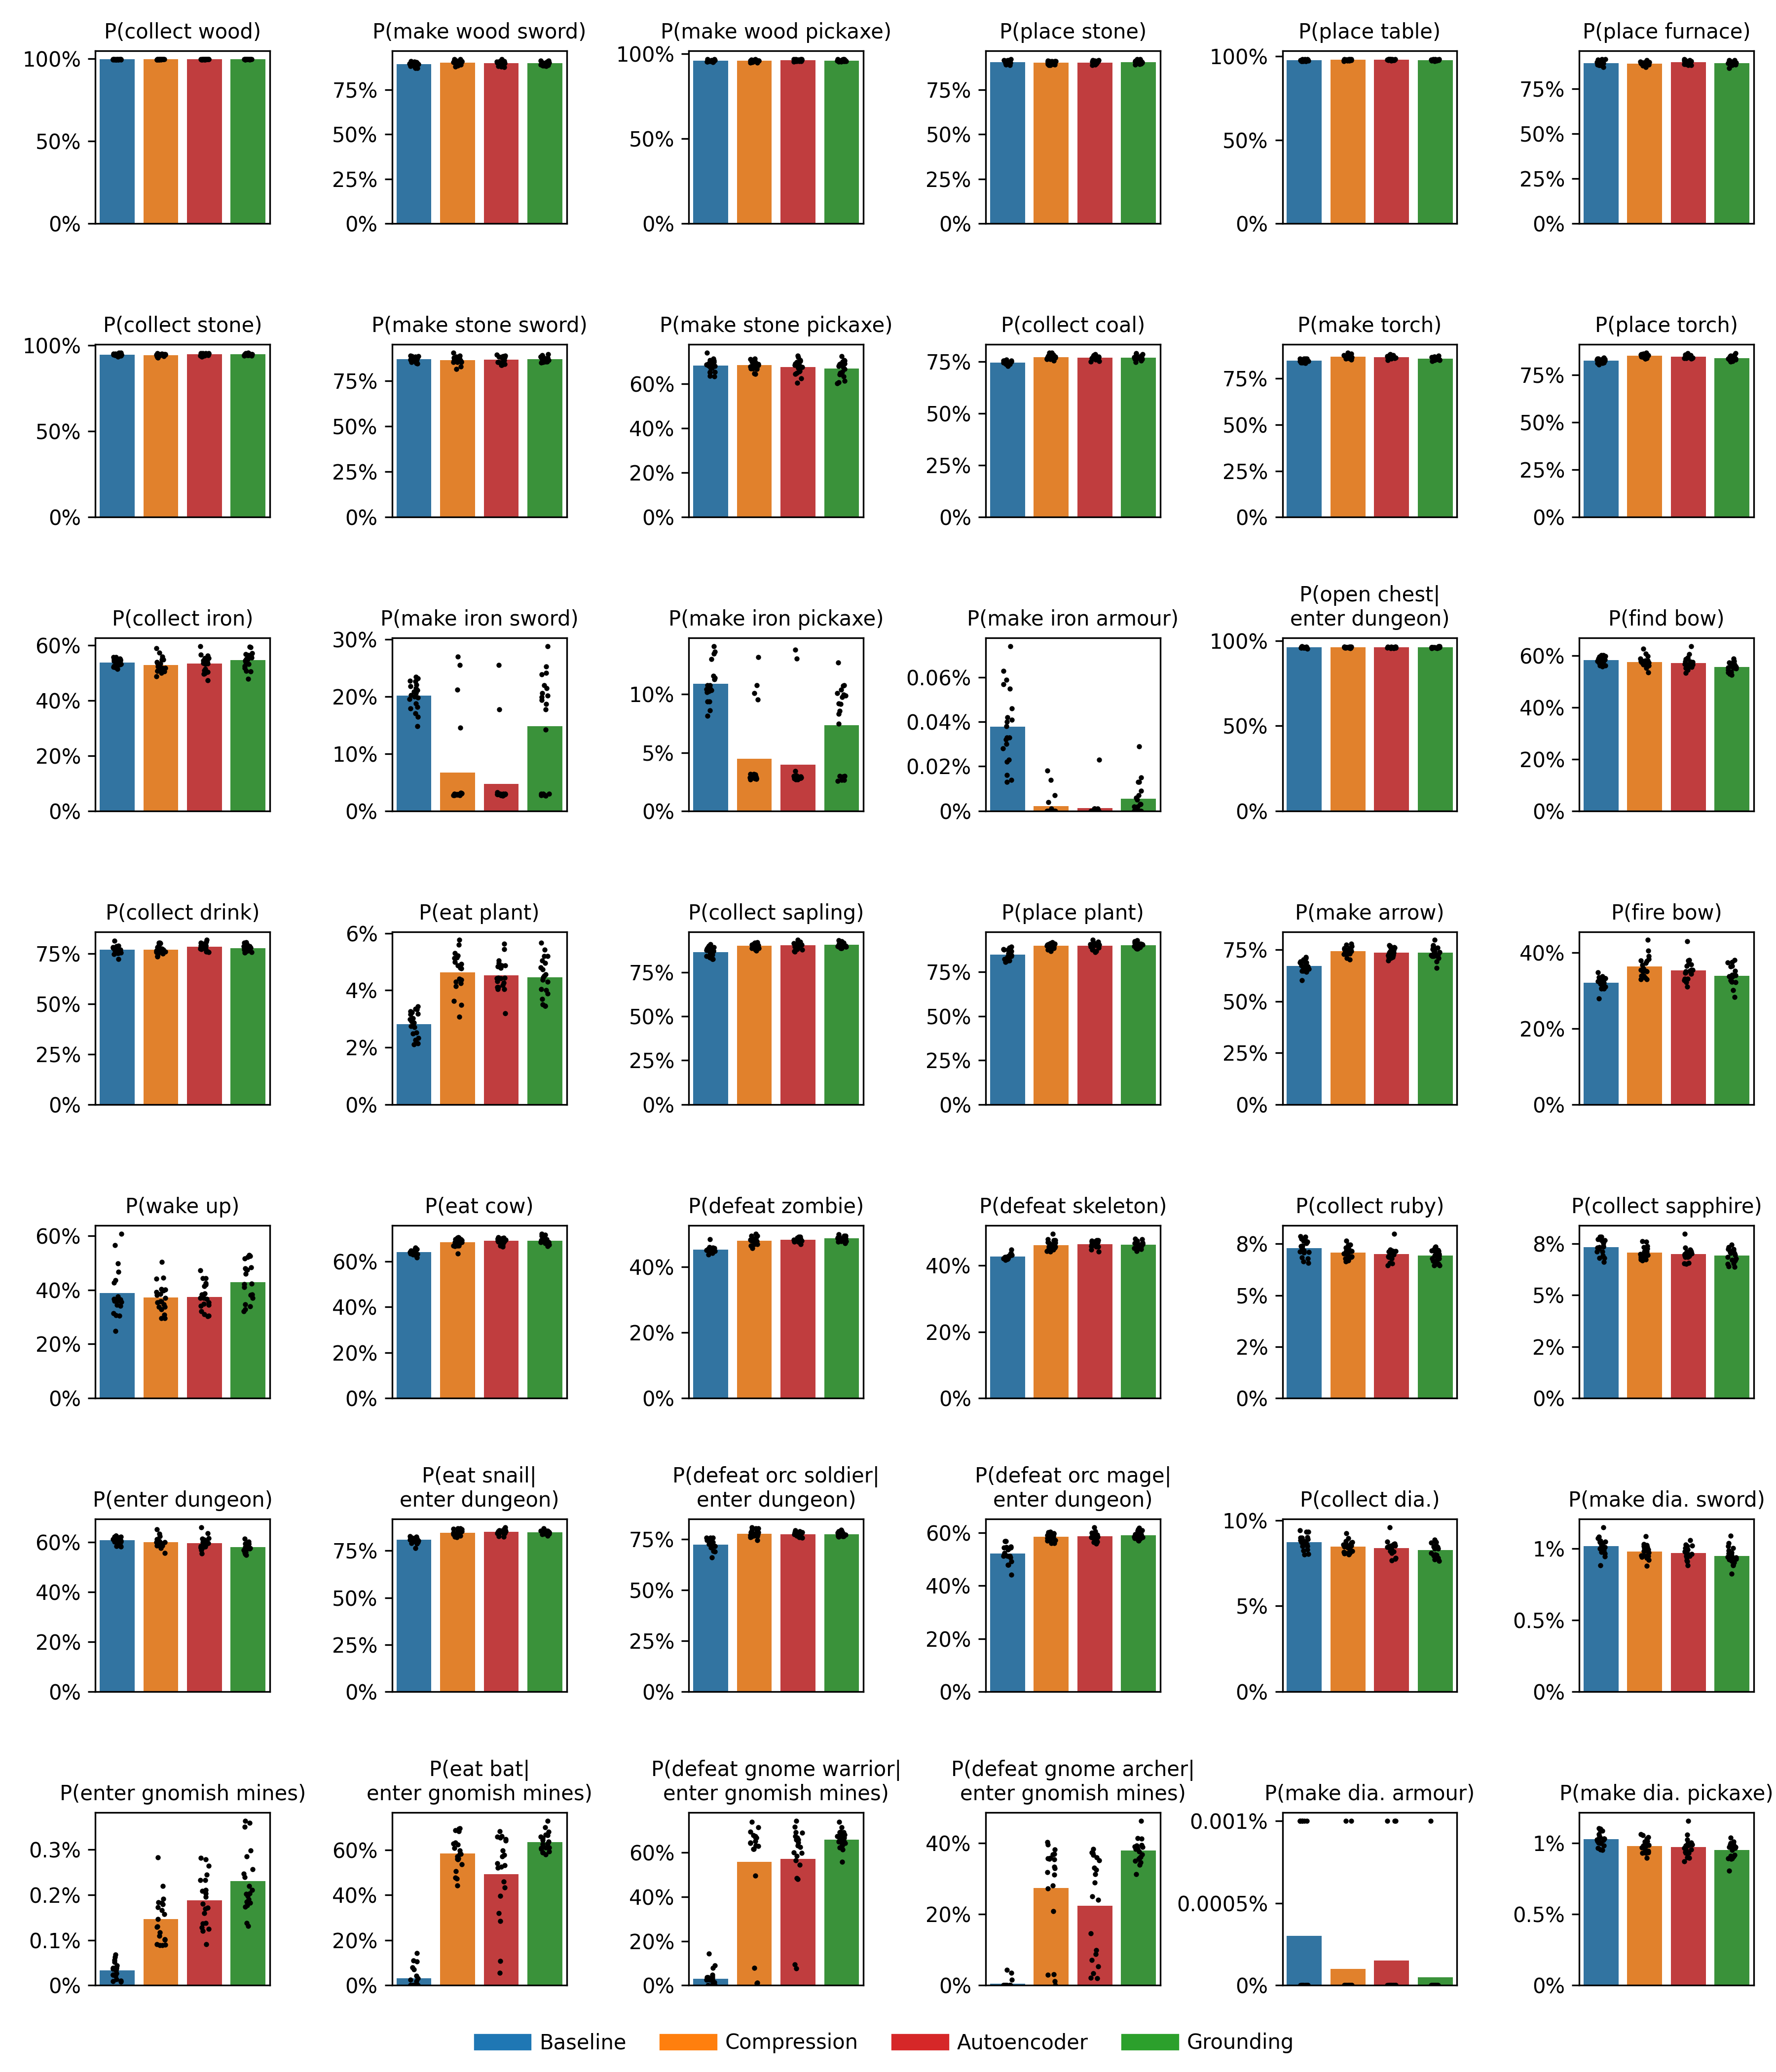
\includegraphics[width=\linewidth]{include/abtest.png}}
\end{figure}

\begin{table}[htbp]
\centering
\small
\setlength{\tabcolsep}{4pt}
\caption{Statistical tests}
\label{tab:tests}
\vspace{10pt}
\begin{tabular}{lcrcrcrc}
\toprule
& \textbf{Baseline} & \multicolumn{2}{c}{\textbf{Compression}} & \multicolumn{2}{c}{\textbf{Autoencoder}} & \multicolumn{2}{c}{\textbf{Grounding}} \\
\textbf{Metric} & $\mu\pm\sigma$ (\%) & $\Delta$p.p. & $p$-val & $\Delta$p.p. & $p$-val & $\Delta$p.p. & $p$-val \\
\midrule
P(collect wood)          & 99.53 $\pm$ 0.11 &      0.06  & 0.9781 &      0.09  & 0.3332 &      0.05  & 1.0000 \\
P(make wood sword)       & 89.19 $\pm$ 1.05 &      1.00  & 0.1311 &      0.58  & 1.0000 &      0.58  & 1.0000 \\
P(make wood pickaxe)     & 95.80 $\pm$ 0.46 &     -0.01  & 1.0000 &      0.28  & 0.9444 &      0.20  & 1.0000 \\
P(place stone)           & 90.51 $\pm$ 0.80 &     -0.39  & 1.0000 &     -0.25  & 1.0000 &      0.05  & 1.0000 \\
P(place table)           & 97.65 $\pm$ 0.40 &      0.26  & 0.5043 &      0.33  & 0.1420 &      0.14  & 1.0000 \\
P(place furnace)         & 89.46 $\pm$ 1.21 &     -0.30  & 1.0000 &      0.40  & 1.0000 &     -0.01  & 1.0000 \\
P(collect stone)         & 94.61 $\pm$ 0.54 &     -0.27  & 1.0000 &      0.10  & 1.0000 &      0.10  & 1.0000 \\
P(make stone sword)      & 86.87 $\pm$ 1.32 &     -0.34  & 1.0000 &     -0.24  & 1.0000 &      0.21  & 1.0000 \\
P(make stone pickaxe)    & 68.28 $\pm$ 2.62 &      0.15  & 1.0000 &     -0.66  & 1.0000 &     -1.31  & 1.0000 \\
P(collect coal)          & 74.61 $\pm$ 0.79 &  \ub{2.59} & 0.0001 &  \uu{2.29} & 0.0001 &  \uu{2.38} & 0.0001 \\
P(make torch)            & 84.78 $\pm$ 0.77 &  \ub{1.98} & 0.0001 &  \uu{1.87} & 0.0001 &  \uu{1.09} & 0.0091 \\
P(place torch)           & 82.39 $\pm$ 0.98 &  \ub{2.50} & 0.0001 &  \uu{2.21} & 0.0001 &  \uu{1.40} & 0.0112 \\
P(collect iron)          & 53.64 $\pm$ 1.31 &     -0.89  & 1.0000 &     -0.40  & 1.0000 &      0.94  & 1.0000 \\
P(make iron sword)       & 20.16 $\pm$ 2.31 & \uu{-13.42}& 0.0016 & \uu{-15.41}& 0.0001 & \bb{-5.35} & 1.0000 \\
P(make iron pickaxe)     & 10.93 $\pm$ 1.57 & \uu{-6.44} & 0.0002 & \uu{-6.98} & 0.0002 & \ub{-3.58} & 0.0086 \\
P(make iron armour)      &  0.04 $\pm$ 0.02 & \uu{-0.04} & 0.0001 & \uu{-0.04} & 0.0001 & \ub{-0.03} & 0.0001 \\
P(find bow)              & 58.26 $\pm$ 1.38 & \bb{-0.70} & 1.0000 &     -1.13  & 0.3332 & \uu{-2.61} & 0.0008 \\
P(make arrow)            & 67.17 $\pm$ 2.59 &  \ub{7.21} & 0.0001 &  \uu{6.45} & 0.0001 &  \uu{6.36} & 0.0001 \\
P(fire bow)              & 32.12 $\pm$ 1.50 &  \ub{4.24} & 0.0001 &  \uu{3.28} & 0.0010 &  \uu{1.89} & 0.0364 \\
P(collect drink)         & 76.88 $\pm$ 1.80 &      0.00  & 1.0000 &      1.37  & 0.1829 &      0.78  & 1.0000 \\
P(collect sapling)       & 86.26 $\pm$ 2.56 &  \uu{3.74} & 0.0003 &  \uu{3.94} & 0.0005 &  \ub{4.22} & 0.0001 \\
P(place plant)           & 84.85 $\pm$ 2.62 &  \uu{4.95} & 0.0001 &  \uu{5.15} & 0.0001 &  \ub{5.26} & 0.0001 \\
P(eat plant)             & 02.81 $\pm$ 0.44 &  \ub{1.81} & 0.0001 &  \uu{1.71} & 0.0001 &  \uu{1.65} & 0.0001 \\
P(wake up)               & 38.81 $\pm$ 8.64 &     -1.61  & 1.0000 &     -1.35  & 1.0000 &      4.04  & 0.7912 \\
P(eat cow)               & 64.08 $\pm$ 1.03 &  \uu{4.33} & 0.0001 &  \uu{4.98} & 0.0001 &  \ub{5.05} & 0.0001 \\
P(defeat zombie)         & 45.29 $\pm$ 0.90 &  \uu{2.78} & 0.0001 &  \uu{2.99} & 0.0001 &  \ub{3.41} & 0.0001 \\
P(defeat skeleton)       & 42.70 $\pm$ 0.77 &  \uu{3.47} & 0.0001 &  \ub{3.72} & 0.0001 &  \uu{3.50} & 0.0001 \\
P(enter dungeon)         & 60.60 $\pm$ 1.42 & \bb{-0.79} & 1.0000 &     -1.17  & 0.2903 & \uu{-2.74} & 0.0004 \\
P(open chest|dungeon)    & 96.14 $\pm$ 0.28 &      0.09  & 1.0000 &     -0.01  & 1.0000 &      0.04  & 1.0000 \\
P(eat snail|dungeon)     & 80.77 $\pm$ 1.45 &  \uu{3.78} & 0.0001 &  \ub{4.24} & 0.0001 &  \uu{4.04} & 0.0001 \\
P(defeat orc soldier|...)& 72.20 $\pm$ 2.39 &  \ub{5.40} & 0.0001 &  \uu{5.07} & 0.0001 &  \uu{5.23} & 0.0001 \\
P(defeat orc mage|...)   & 52.24 $\pm$ 3.23 &  \uu{6.19} & 0.0001 &  \uu{6.36} & 0.0001 &  \ub{6.82} & 0.0001 \\
P(enter g. mines)        &  0.03 $\pm$ 0.02 &  \uu{0.11} & 0.0001 &  \uu{0.16} & 0.0001 &  \ub{0.20} & 0.0001 \\
P(eat bat|mines)         &  3.14 $\pm$ 4.43 & \uu{55.35} & 0.0001 & \uu{46.19} & 0.0001 & \ub{60.26} & 0.0001 \\
P(defeat g. warrior|...) &  2.96 $\pm$ 3.66 & \uu{52.78} & 0.0001 & \uu{54.11} & 0.0001 & \ub{62.90} & 0.0001 \\
P(defeat g. archer|...)  &  0.48 $\pm$ 1.22 & \uu{26.93} & 0.0001 & \uu{22.00} & 0.0001 & \ub{37.44} & 0.0001 \\
P(collect ruby)          &  7.30 $\pm$ 0.38 &     -0.23  & 0.9584 &     -0.30  & 0.1852 &     -0.37  & 0.0635 \\
P(collect sapphire)      &  7.33 $\pm$ 0.35 & \bb{-0.26} & 0.3000 &     -0.33  & 0.0512 & \uu{-0.41} & 0.0175 \\
P(collect diamond)       &  8.72 $\pm$ 0.39 & \bb{-0.27} & 0.5005 &     -0.35  & 0.0846 & \uu{-0.47} & 0.0183 \\
P(make dia. sword)       &  1.02 $\pm$ 0.05 & \bb{-0.04} & 0.2832 &     -0.05  & 0.0581 & \uu{-0.07} & 0.0112 \\
P(make dia. pickaxe)     &  1.03 $\pm$ 0.04 & \bb{-0.05} & 0.0867 & \uu{-0.06} & 0.0213 & \uu{-0.08} & 0.0021 \\
P(make dia. armour)      &  3e-4 $\pm$ 5e-4 &   -2.0e-4  & 1.0000 &    -1.5e-4 & 1.0000 &   -2.5e-4  & 0.6294 \\
\bottomrule
\end{tabular}
\end{table}

\end{document}
